\par\Needspace{10\baselineskip}
\section{路径积分}
\label{sec:multivariable-path-integration}

细线的质量由线密度和长度决定，力沿路线做功还取决于位移方向。
两种问题的积分位置都是一条路径，但被积对象不同：线密度是标量函数，力是向量场。
第一类路径积分用弧长累计标量值，第二类路径积分先取向量场与有向位移的内积，再累计这个标量。
两者都要先规定路径的参数化；下面分别说明各自的定义、可积要求、性质和计算方法，最后研究第二类路径积分何时只依赖端点。所有参数积分均为勒贝格积分\scite{math-openstax-calculus3}。

\subsection{参数路径与弧长}
\label{sec:multivariable-line-integrals}

路径既要说明走过哪些位置，也要说明行进次序。弧长则把参数增量换成实际路程，为第一类路径积分提供权重。

\subsubsection{路径的定义}

\paragraph{参数化路径}

同一个几何点集可以按不同速度、不同方向走过，甚至被重复走过。用区间到空间的连续映射，可以把这些行进信息一并保留下来。
\begin{definition}[路径]
设$a<b$。连续映射$\gamma:[a,b]\to\mathbb R^d$称为一条\term{路径}（path），$\gamma(a)$和$\gamma(b)$分别为起点和终点；若两者相等，称为闭路径。
集合$C=\gamma([a,b])$称为路径的像。
\end{definition}

参数$t$指定行进次序，像集$C$只记录经过的位置。例如$\gamma(t)=(t,t)^\top$、$0\leq t\leq1$从$(0,0)$走到$(1,1)$；$\eta(u)=(u/2,u/2)^\top$、$0\leq u\leq2$沿同一方向走过同一条线段。
二者的速度不同，但没有改变行进次数。相反，沿同一线段往返的路径不能只凭这个线段的像集确定累计量。

\paragraph{分段光滑路径}

折线在转角处没有唯一切线，但每一条线段仍可计算速度。为了把这些路径也纳入计算，允许在有限个参数点处分段。
\begin{definition}[分段光滑路径]
若存在分割$a=t_0<t_1<\cdots<t_n=b$，使$\gamma$在每个$[t_{j-1},t_j]$上为$C^1$映射，称$\gamma$为分段$C^1$路径，也称分段光滑路径。
若每段内部还满足$\gamma'(t)\neq\bm0$，称该路径分段正则。
\end{definition}

这里每一段的导数都连续延拓到该段端点，相邻两段的端点导数不必相同。
本节路径积分均在分段$C^1$路径上定义，折点处的有限个取值不影响参数积分；单位切向量只在速度非零处使用。

\subsubsection{路径的长度}

\paragraph{弧长}

用路径上依次选出的点连接成折线，可以从下方估计实际路程。细分后取所有这类折线长度的上确界，就得到不依赖所选分割的长度。
\begin{definition}[路径的弧长]
路径$\gamma:[a,b]\to\mathbb R^d$的弧长定义为
\[
 \ell(\gamma)=\sup_{a=t_0<\cdots<t_n=b}
 \sum_{j=1}^n\lVert\gamma(t_j)-\gamma(t_{j-1})\rVert_2.
\]
上确界取遍$[a,b]$的全部有限分割；若此值有限，称路径可求长。
\end{definition}

对光滑路径，小段位移由速度乘参数增量近似。因此弧长可以由速度的大小累计，得到下面的计算公式。
\begin{theorem}[分段光滑路径的弧长]
若$\gamma:[a,b]\to\mathbb R^d$分段$C^1$，则它可求长，且
\[
 \ell(\gamma)=\int_a^b\lVert\gamma'(t)\rVert_2\,\mathrm dt.
\]
\end{theorem}
\begin{proof}
先在一段$C^1$区间上证明。由各坐标的一元基本定理，
$\gamma(v)-\gamma(u)=\int_u^v\gamma'(t)\,\mathrm dt$，这里向量积分表示对各分量分别积分。将此等式与弦方向的单位向量取内积，再用Cauchy--Schwarz不等式，可知每段弦长不超过$\int_u^v\lVert\gamma'(t)\rVert_2\,\mathrm dt$。弦为零时这个不等式直接成立。相加后，任意内接折线的长度都不超过速度范数的积分。

反过来，$\gamma'$在紧区间上一致连续。若分割足够细，使每个小区间上$\gamma'$的振幅小于$\varepsilon$，并在其中取一点$\xi_j$，则弦向量与$\gamma'(\xi_j)(t_j-t_{j-1})$的距离不超过$\varepsilon(t_j-t_{j-1})$。
同一小区间上$\lVert\gamma'\rVert_2$的积分与$\lVert\gamma'(\xi_j)\rVert_2(t_j-t_{j-1})$的差也不超过这个数。
因此速度积分与该折线长度的差不超过$2\varepsilon(b-a)$。令$\varepsilon\downarrow0$，得到反向不等式。分段$C^1$的情形对各段相加即可。
\end{proof}

记$s(t)=\int_a^t\lVert\gamma'(u)\rVert_2\,\mathrm du$为截至参数$t$的累计路程，常将长度权重写为
$\mathrm ds=\lVert\gamma'(t)\rVert_2\,\mathrm dt$。例如前述对角线段的速度为$(1,1)^\top$，长度为$\sqrt2$；两个坐标分别变化$1$，并不意味着实际长度为$2$。

\subsection{第一类路径积分}

第一类路径积分的被积对象是沿路径给定的标量函数，例如线密度。每一小段的贡献是函数值乘实际弧长，因此不需要指定力或其他向量场。

\subsubsection{定义与可积性}

\paragraph{按弧长的积分}

把路径分成小段并累计函数值乘小段长度，会得到弧长权重$\lVert\gamma'(t)\rVert_2$。用这个权重定义积分，也允许处理沿路径可测而不连续的标量函数。
\begin{definition}[第一类路径积分]
设$\gamma:[a,b]\to\mathbb R^d$分段$C^1$，$h:C\to\mathbb R$，其中$C=\gamma([a,b])$，且$h\circ\gamma$在参数区间上勒贝格可测。
若$h\geq0$，定义\term{第一类路径积分}（scalar line integral）为
\begin{equation}
 \int_\gamma h\,\mathrm ds
 =\int_a^b h(\gamma(t))\lVert\gamma'(t)\rVert_2\,\mathrm dt,
 \label{eq:analysis-scalar-line-integral}
\end{equation}
允许取$+\infty$。对一般有符号$h$，本节称它沿$\gamma$可积，是指
\[
 \int_a^b |h(\gamma(t))|\lVert\gamma'(t)\rVert_2\,\mathrm dt<\infty;
\]
此时由正负部分之差定义积分，式~\eqref{eq:analysis-scalar-line-integral}仍成立并取有限值。
\end{definition}

$h=1$给出弧长；非负线密度的积分给出细线质量。若$h$在紧像集$C$上连续，它有界，因而绝对积分不超过$\sup_C|h|\,\ell(\gamma)<\infty$。连续性是方便的充分条件，并非定义本身的要求。

这里必须知道路径上的实际取值，以及它与参数复合后的可测性。仅有环境区域中的勒贝格可积性不能替代这个要求。
例如$h(x,y)=\mathbb I\{y=0\}$在平面几乎处处为零，但沿$\gamma(t)=(t,0)$、$0\leq t\leq1$的弧长积分为$1$。
面积零测集仍可有正长度，不能从平面函数的几乎处处等价类直接读出线积分。

\subsubsection{积分的基本性质}

下面的有符号公式都假设相应标量函数沿所讨论路径可积。将参数公式代入一元勒贝格积分的性质，就能逐项得到这些结论。

\paragraph{加法}

若$h,k$沿$\gamma$可积，则$h+k$也沿$\gamma$可积，且
\[
 \int_\gamma(h+k)\,\mathrm ds=\int_\gamma h\,\mathrm ds+\int_\gamma k\,\mathrm ds.
\]
绝对可积性由$|h+k|\leq|h|+|k|$保证。

\paragraph{减法}

对同一组可积函数，将$k$换成其相反函数，得到
\[
 \int_\gamma(h-k)\,\mathrm ds=\int_\gamma h\,\mathrm ds-\int_\gamma k\,\mathrm ds.
\]
两边均为有限数，不涉及无穷相消。

\paragraph{常数倍}

若$c\in\mathbb R$且$h$沿$\gamma$可积，则
\[
 \int_\gamma ch\,\mathrm ds=c\int_\gamma h\,\mathrm ds.
\]
这表示将每一小段上的密度同时放大$c$倍，累计量也按相同比例变化。

\paragraph{路径拼接}

若$\gamma_1$的终点是$\gamma_2$的起点，记依次走过两条路径的拼接为$\gamma_1*\gamma_2$。沿两条路径分别可积时，
\[
 \int_{\gamma_1*\gamma_2}h\,\mathrm ds
 =\int_{\gamma_1}h\,\mathrm ds+\int_{\gamma_2}h\,\mathrm ds.
\]
参数区间的可加性给出这个等式；若某段被重复走过，它的贡献也会重复计入。

\paragraph{重参数化与方向无关}

设$t=\eta(u)$是两个参数区间之间单调、端点相配的分段$C^1$微分同胚。链式法则给出
$\lVert(\gamma\circ\eta)'(u)\rVert_2=\lVert\gamma'(\eta(u))\rVert_2|\eta'(u)|$，再用一元换元可得
\[
 \int_{\gamma\circ\eta}h\,\mathrm ds=\int_\gamma h\,\mathrm ds.
\]
无论$\eta$递增还是递减，绝对值都保留非负弧长权重，因此反向行进不改变第一类积分。这个结论只改变行进速度或方向，不改变行进次数。

\paragraph{单调性}

若$h\leq k$在路径上成立，则非负弧长权重保证
\[
 \int_\gamma h\,\mathrm ds\leq\int_\gamma k\,\mathrm ds.
\]
这里比较的是同一路径上的两个标量函数。

\paragraph{绝对值不等式}

由一元积分的绝对值不等式可得
\[
 \left|\int_\gamma h\,\mathrm ds\right|
 \leq\int_\gamma|h|\,\mathrm ds
 \leq\sup_C|h|\,\ell(\gamma).
\]
最后一个不等式在$h$有界时适用。它用路径长度和函数的大小控制累计量。

\subsubsection{积分的计算}

计算时先参数化路径，再将标量函数乘速度范数，转为一元积分；折点两侧逐段相加。
例如在线段$\gamma(t)=(t,t)^\top$、$0\leq t\leq1$上取$h(x,y)=x+y$，得到
\[
 \int_\gamma h\,\mathrm ds=\int_0^1 2t\sqrt2\,\mathrm dt=\sqrt2.
\]
累计的是沿线的函数值，而非线段下方的平面面积。

沿$x$递增的图像路径$\gamma(x)=(x,\psi(x))^\top$，$a\leq x\leq b$，若$\psi$为$C^1$，则
\[
 \int_\gamma h\,\mathrm ds
 =\int_a^b h(x,\psi(x))\sqrt{1+\psi'(x)^2}\,\mathrm dx.
\]
根号是图像路径的速度范数，不能省略为单独的$\mathrm dx$权重。

\subsection{第二类路径积分}

做功问题中，被积对象变成向量场：每个位置给出一个向量。位移方向改变时，向量在该方向上的分量可能变号，因此需要有向累计。

\subsubsection{定义与可积性}

\paragraph{向量场}

要在空间中描述力，必须为每个位置同时给出大小和方向。定义域与输出空间具有相同维数的向量值映射，正适合记录这种信息。
\begin{definition}[向量场]
设$U\subseteq\mathbb R^d$。映射$\bm F:U\to\mathbb R^d$称为$U$上的\term{向量场}（vector field）。
\end{definition}

向量场的输入是位置，输出是该位置的一个向量。例如$\bm F(x,y)=(-y,x)^\top$给出的向量与以原点为圆心的圆相切。
若它表示力，小段做功是场值与位移的内积，只有沿位移方向的分量参与做功。

\paragraph{有向线积分}

沿参数路径的小段有向位移近似为$\gamma'(t)\,\mathrm dt$。将场值与这个位移取内积，得到一个可以在参数区间上累计的标量函数。
\begin{definition}[第二类路径积分]
设$\gamma:[a,b]\to U$分段$C^1$，$\bm F:U\to\mathbb R^d$为向量场。
若$\bm F\circ\gamma$的每个分量勒贝格可测，且$t\mapsto\bm F(\gamma(t))^\top\gamma'(t)$绝对可积，定义\term{第二类路径积分}（vector line integral）为
\begin{equation}
 \int_\gamma\bm F\mathbin{\cdot}\mathrm d\bm r
 =\int_a^b\bm F(\gamma(t))^\top\gamma'(t)\,\mathrm dt.
 \label{eq:analysis-vector-line-integral}
\end{equation}
\end{definition}

在平面中，$\bm F=(P,Q)^\top$时写为$\int_\gamma P\,\mathrm dx+Q\,\mathrm dy$；三维中再加$R\,\mathrm dz$。
若$\bm F$在路径像集上连续，复合函数在各段连续，从而上述参数积分绝对可积。
更一般地，可测性以及$\int_a^b\lVert\bm F(\gamma(t))\rVert_2\lVert\gamma'(t)\rVert_2\,\mathrm dt<\infty$也是充分条件，因为内积的绝对值不超过范数之积。

速度非零处的单位切向量为$\bm\tau=\gamma'/\lVert\gamma'\rVert_2$，所以
$\bm F\cdot\mathrm d\bm r=(\bm F^\top\bm\tau)\,\mathrm ds$。
第二类积分累计的是向量场的切向分量；沿闭路径累计时也称\term{环流}（circulation）。它可以转写为一个标量的弧长积分，但这个标量随所选行进方向改变。


图~\ref{fig:analysis-process-line-density-work}用同一条线段对照弧长累计与有向位移累计，避免把速度范数和内积混用。
\begin{figure}[!htbp]
 \centering
 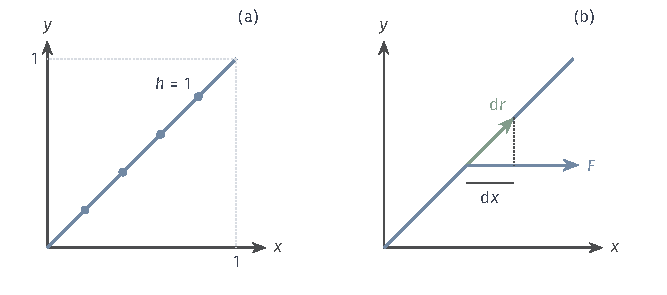
\includegraphics[width=112mm]{figures/01-mathematical-preliminaries-upper/01-mathematical-language-combinatorics-analysis-optimization/tikz/chapter3-concept-processes/line-density-work.pdf}
 \caption{路径均为$\gamma(t)=(t,t)^\top$，$0\leq t\leq1$。(a) 常数线密度$h=1$按弧长累计，得到$\sqrt2$。(b) 常向量场$F=(1,0)^\top$只取位移的水平分量，做功为$1$；图中$\mathrm dx$是$\mathrm dr$的水平投影。相同路径、不同被积对象和权重给出不同积分。}
 \label{fig:analysis-process-line-density-work}
\end{figure}

\subsubsection{积分的基本性质}

下列公式均由内积和一元勒贝格积分的相应性质得到，并要求涉及的有向积分存在且有限。

\paragraph{加法}

若$\bm F$和$\bm G$沿$\gamma$可积，则
\[
 \int_\gamma(\bm F+\bm G)\cdot\mathrm d\bm r
 =\int_\gamma\bm F\cdot\mathrm d\bm r+\int_\gamma\bm G\cdot\mathrm d\bm r.
\]
这里相加的是两个向量场，内积后才得到被积标量。

\paragraph{减法}

将$\bm G$换成其相反场，得到
\[
 \int_\gamma(\bm F-\bm G)\cdot\mathrm d\bm r
 =\int_\gamma\bm F\cdot\mathrm d\bm r-\int_\gamma\bm G\cdot\mathrm d\bm r.
\]
可积性使两个方向的累计量都有限，因而可以相减。

\paragraph{常数倍}

对实数$c$，有
\[
 \int_\gamma c\bm F\cdot\mathrm d\bm r
 =c\int_\gamma\bm F\cdot\mathrm d\bm r.
\]
系数只改变场的大小和符号，不改变路径的几何形状与方向。

\paragraph{路径拼接}

若$\gamma_1$和$\gamma_2$首尾相接，则
\[
 \int_{\gamma_1*\gamma_2}\bm F\cdot\mathrm d\bm r
 =\int_{\gamma_1}\bm F\cdot\mathrm d\bm r
 +\int_{\gamma_2}\bm F\cdot\mathrm d\bm r.
\]
这使分段光滑路径可以逐段计算；每段都必须保留该次行进的方向。

\paragraph{方向反转}

记反向路径为$\gamma^{-}(u)=\gamma(a+b-u)$，$a\leq u\leq b$。它的速度是原速度的相反向量，一元换元因此给出
\[
 \int_{\gamma^{-}}\bm F\cdot\mathrm d\bm r
 =-\int_\gamma\bm F\cdot\mathrm d\bm r.
\]
这与第一类积分反向后不变相区别：长度始终非负，有向位移则改变符号。

\paragraph{重参数化}

若$t=\eta(u)$为端点相配、严格递增的分段$C^1$微分同胚，则
$(\gamma\circ\eta)'(u)=\gamma'(\eta(u))\eta'(u)$。在参数公式中应用换元，得到
\[
 \int_{\gamma\circ\eta}\bm F\cdot\mathrm d\bm r
 =\int_\gamma\bm F\cdot\mathrm d\bm r.
\]
严格递减的重参数化会反转方向，因而积分变号。方向相同的不同速度不会改变积分，重复行进的次数却仍会被保留。

\paragraph{绝对值不等式}

由积分的三角不等式和内积的Cauchy--Schwarz不等式可得
\[
 \left|\int_\gamma\bm F\cdot\mathrm d\bm r\right|
 \leq\int_\gamma\lVert\bm F\rVert_2\,\mathrm ds.
\]
右侧有限时，它为做功或环流的绝对值提供上界；若右侧为$+\infty$，不等式仍成立，但不能用来证明左侧有限。

\subsubsection{积分的计算}

参数化以后，第二类积分把场值与速度取内积，不乘速度范数。例如常向量场$\bm F=(1,0)^\top$沿前述对角线段的积分为
\[
 \int_0^1(1,0)\cdot(1,1)\,\mathrm dt=1.
\]
同一路径的长度为$\sqrt2$，两种结果对应不同的被积对象和局部权重。

对平面图像路径$\gamma(x)=(x,\psi(x))^\top$、$a\leq x\leq b$，$\bm F=(P,Q)^\top$时有
\[
 \int_\gamma\bm F\cdot\mathrm d\bm r
 =\int_a^b\bigl[P(x,\psi(x))+Q(x,\psi(x))\psi'(x)\bigr]\,\mathrm dx.
\]
下面固定起终点比较不同路径，观察这个积分是否还会依赖路线。

\begin{example}[半圆和直径]
\label{ex:analysis-path-integral-comparison}
取$\gamma(t)=(\cos t,\sin t)$，$0\leq t\leq\pi$。它从$(1,0)$沿上半圆走到$(-1,0)$，速度范数为$1$，故$\int_\gamma1\,\mathrm ds=\pi$。
对常场$(1,0)^\top$，积分为$\int_0^\pi-\sin t\,\mathrm dt=-2$，恰等于函数$\phi(x,y)=x$的端点值之差。
对旋转场$\bm F=(-y,x)^\top$，代入得$\bm F(\gamma(t))\cdot\gamma'(t)=1$，故积分为$\pi$。
沿同起终点的直径$\eta(t)=(1-2t,0)$、$0\leq t\leq1$，这个旋转场与位移的内积恒为零，积分为$0$。
光滑向量场的线积分也可能依赖路线。沿完整单位圆逆时针一周，旋转场的积分则为$2\pi$。
\end{example}


图~\ref{fig:analysis-process-rotation-field-paths}显示半圆与直径虽然端点相同，旋转场的做功却不同。
\begin{figure}[!htbp]
 \centering
 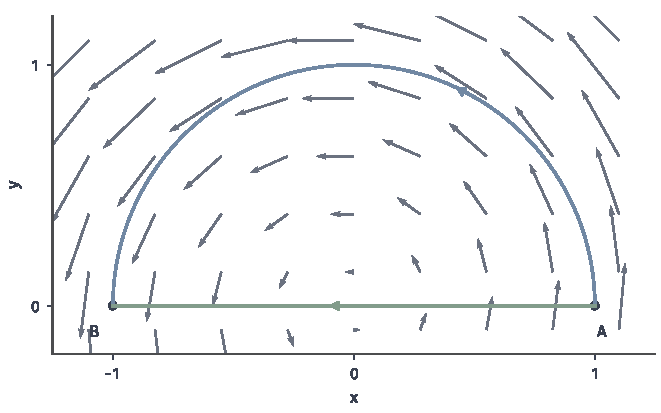
\includegraphics[width=112.0mm]{figures/01-mathematical-preliminaries-upper/01-mathematical-language-combinatorics-analysis-optimization/matplotlib/chapter3-concept-processes/rotation-field-paths.pdf}
 \caption{灰箭头为旋转场$F=(-y,x)^\top$，箭头长度统一缩放为实际场值的$1/4$。两条路径都从$A=(1,0)$到$B=(-1,0)$：蓝色上半圆与场同向，积分为$\pi$；绿色直径上场与位移垂直，积分为零。光滑性及相同端点不保证路径无关，下一小节将说明势函数给出的条件。}
 \label{fig:analysis-process-rotation-field-paths}
\end{figure}

\subsection{路径无关与势函数}
\label{sec:multivariable-potential-path-independence}

一般向量场的积分可能依赖整条路线。若向量场来自某个标量函数的梯度，链式法则就能把沿途累计化为端点变化；接下来分别说明这一结论、它的逆向判别以及定义域所需的条件。

\subsubsection{势函数与路径积分}

\paragraph{势函数}

寻找一个以向量场为梯度的标量函数，可以把做功解释成这个标量的变化。这样一个函数把每点的向量与整体端点差联系起来。
\begin{definition}[势函数]
设$U\subseteq\mathbb R^d$为非空开集，$\bm F:U\to\mathbb R^d$连续。
若存在$\phi\in C^1(U)$使$\bm F=\nabla\phi$，称$\phi$为$\bm F$的\term{势函数}（potential function），称$\bm F$为梯度场，也称保守场。
\end{definition}

例如$\phi(x,y)=x^2+y^2$给出$\bm F(x,y)=(2x,2y)^\top$；给势函数加常数不会改变该场。

\paragraph{路径积分基本定理}

将势函数与路径复合，就得到一个一元函数。它的导数恰是第二类路径积分中的被积函数，因此一元基本定理能恢复端点差。
\begin{theorem}[路径积分基本定理]
设$U\subseteq\mathbb R^d$为开集，$\phi\in C^1(U)$，$\gamma:[a,b]\to U$分段$C^1$。则
\begin{equation}
  \int_{\gamma}\nabla\phi\mathbin{\cdot}\mathrm{d}\bm{r}
  =\phi(\gamma(b))-\phi(\gamma(a)).
\label{eq:analysis-line-integral-gradient}
\end{equation}
\end{theorem}
\begin{proof}
在每个光滑参数段上，链式法则给出
\[
 (\phi\circ\gamma)'(t)=\nabla\phi(\gamma(t))^\top\gamma'(t).
\]
这个导数连续，所以对该段使用一元基本定理，积分等于该段两端的函数值之差。
对所有段相加，中间端点项逐一抵消，得到所述等式。
\end{proof}

因此梯度场的积分只依赖端点，任意闭路径上的积分都为零。方向反转使端点差变号，与前面的有向积分性质一致。

\subsubsection{路径无关的等价判别}

\paragraph{路径无关}

为了比较同一对端点间的不同路线，先要求域内任意两点能够由路径连接。欧氏开集若路径连通，任意两点之间也能选择域内的分段光滑路径。
\begin{definition}[路径无关]
设$U\subseteq\mathbb R^d$为非空、开且路径连通的集合，$\bm F:U\to\mathbb R^d$连续。
若对任意$\bm a,\bm b\in U$及域内从$\bm a$到$\bm b$的任意两条分段$C^1$路径，第二类路径积分都相等，称$\bm F$的路径积分与路径无关。
\end{definition}

势函数已给出路径无关的充分条件。反过来，若累计只由端点决定，就可以固定起点，用累计值定义势函数。
\begin{theorem}[路径无关的等价条件]
设$U\subseteq\mathbb R^d$非空、开且路径连通，$\bm F:U\to\mathbb R^d$连续。下列条件等价：
\begin{enumerate}
 \item 存在$\phi\in C^1(U)$使$\nabla\phi=\bm F$；
 \item $\bm F$的路径积分与路径无关；
 \item 域内每条分段$C^1$闭路径的积分都为零。
\end{enumerate}
\end{theorem}
\begin{proof}
条件1由路径积分基本定理推出条件2；条件2与常值闭路径比较，推出条件3。
若条件3成立，将两条同端点路径中的第二条反向，与第一条拼成闭路径，便得到两条原路径积分相等，因此条件3推出条件2。

最后假设条件2。固定$\bm a\in U$，用从$\bm a$到$\bm x$的路径积分定义$\phi(\bm x)$。
路径无关保证定义不依赖所选路线。由于$U$开，在$\bm x$附近可以沿第$j$个坐标追加一条足够短的线段，于是
\[
 \phi(\bm x+h\bm e_j)-\phi(\bm x)
 =\int_0^h F_j(\bm x+t\bm e_j)\,\mathrm dt.
\]
$F_j$连续，右侧除以$h$后趋于$F_j(\bm x)$，所以$\partial_j\phi=F_j$。
所有偏导数均连续，故$\phi\in C^1(U)$，得到条件1。
\end{proof}

\subsubsection{势函数存在的微分判别}

\paragraph{交叉偏导相等的必要条件}

已知势函数时，向量场各分量就是它的一阶偏导数。如果向量场本身为$C^1$，势函数便具有连续二阶偏导，混合偏导交换会给出可直接检查的条件。
\begin{theorem}[保守场的必要条件]
设$U\subseteq\mathbb R^d$为开集，$\bm F\in C^1(U;\mathbb R^d)$。
若$\bm F=\nabla\phi$，其中$\phi\in C^1(U)$，则对所有$i,j$和$\bm x\in U$，有
\[
 \partial_iF_j(\bm x)=\partial_jF_i(\bm x).
\]
\end{theorem}
\begin{proof}
由$\partial_j\phi=F_j\in C^1(U)$可知$\phi\in C^2(U)$，因此
$\partial_iF_j=\partial_i\partial_j\phi=\partial_j\partial_i\phi=\partial_jF_i$。
\end{proof}

\paragraph{星形域上的充分条件}

交叉偏导只比较局部变化，还需要域的条件才能据此构造全局势函数。一个便于直接计算的设定是星形开集：存在$\bm a\in U$，使从$\bm a$到每个$\bm x\in U$的整条线段都在$U$内；凸开集满足这一条件。
\begin{theorem}[星形域上势函数的构造]
设$U\subseteq\mathbb R^d$为关于$\bm a$星形的开集，$\bm F\in C^1(U;\mathbb R^d)$，且对所有$i,j$有$\partial_iF_j=\partial_jF_i$。则
\[
 \phi(\bm x)=\int_0^1\bm F(\bm a+t(\bm x-\bm a))^\top(\bm x-\bm a)\,\mathrm dt
\]
属于$C^1(U)$且满足$\nabla\phi=\bm F$。因此$\bm F$的路径积分与路径无关。
\end{theorem}
\begin{proof}
记$\bm z=\bm x-\bm a$。固定$\bm x$时，从$\bm a$到$\bm x$的线段是$U$内的紧集，因而其一个足够小的紧邻域仍在$U$内。
$\bm F$及其一阶偏导在这个邻域有界，所以可用参数积分的求导结论，在积分号下对第$j$个坐标求导。
交叉偏导条件将被积函数的导数化为
\[
 \begin{aligned}
 F_j(\bm a+t\bm z)+t\sum_i z_i\partial_jF_i(\bm a+t\bm z)
 &=F_j(\bm a+t\bm z)+t\sum_i z_i\partial_iF_j(\bm a+t\bm z)\\
 &=\frac{\mathrm d}{\mathrm dt}\bigl[tF_j(\bm a+t\bm z)\bigr].
 \end{aligned}
\]
积分后得到$\partial_j\phi(\bm x)=F_j(\bm x)$。这些偏导连续，所以$\phi\in C^1(U)$；路径无关由前一定理得到。
\end{proof}

域条件不能省略。例如在穿孔平面$\mathbb R^2\setminus\{\bm0\}$上，
\[
 \bm F(x,y)=\left(-\frac{y}{x^2+y^2},\frac{x}{x^2+y^2}\right)^\top
\]
满足$\partial_yF_1=\partial_xF_2=(y^2-x^2)/(x^2+y^2)^2$，却沿单位圆逆时针一周得到$2\pi$。
这个非零闭路径积分排除了全局势函数。局部导数相容，仍可能无法在整个定义域上把积分写为一个单值势函数的端点差。

\FloatBarrier
